%%\title{Local Reference System}
%  Changed by: Chris ISELIN, 17-Jul-1997 
%  Changed by: Hans Grote, 25-Sep-2002 

\section{Local Reference Systems}

\subsection{\href{straight}{Reference System for Straight Beam
    Elements}} 
In straight elements the local reference system is simply translated by
the length of the element along the local \textit{s}-axis. This is true
for  
\begin{itemize}
   \item \href{drift.html}{Drift space}, 
   \item \href{quadrupole.html}{Quadrupole}, 
   \item \href{sextupole.html}{Sextupole}, 
   \item \href{octupole.html}{Octupole}, 
   \item \href{solenoid.html}{Solenoid}, 
   \item \href{crabcavity.html}{Crab cavity}, 
   \item \href{cavity.html}{RF cavity}, 
   \item \href{separator.html}{Electrostatic separator}, 
   \item \href{kickers.html}{Closed orbit corrector}, 
   \item \href{monitors.html}{Beam position monitor}. 
\end{itemize} 

The corresponding \textit{R}, \textit{S} are 
%%\includegraphics{null}
%RSstraight
\[
R =
 \begin{pmatrix}
  0 \\
  0 \\
  L
 \end{pmatrix}
, \quad
S =
 \begin{pmatrix}
  1 & 0 &  0 \\
  0 & 1 &  0 \\
  0 & 0 &  1
 \end{pmatrix}
.
\]

A rotation of the element about the \textit{S}-axis has no effect on
\textit{R} and \textit{S}, since the rotations of the reference system
before and after the element cancel.  

%%\begin{center}
%%\includegraphics{null}
\begin{figure}[H]
  \centering
	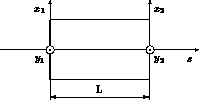
\includegraphics{figures/ref_straight.png}
  \caption{Reference System for Straight Beam Elements}
%\\\textbf{Figure 1:} Reference System for Straight Beam Elements 
\end{figure}



\subsection{\href{rbend}{Reference System for Bending Magnets}}
\href{bend.html}{Bending magnets} have a curved reference orbit. For
both rectangular and sector bending magnets  


%%\includegraphics{null}
%RSbend
\[
R =
 \begin{pmatrix}
  \rho\,(\cos \alpha - 1) \\
  0 \\
  \rho\,\sin \alpha
 \end{pmatrix}
, \quad
S =
 \begin{pmatrix}
  \cos \alpha & 0 &  -\sin \alpha \\
  0 & 1 &  0 \\
  \sin \alpha & 0 &  \cos \alpha
 \end{pmatrix}
,
\]

where alpha is the bend angle. A positive bend angle represents a bend
to the right, i.e. towards negative \textit{x} values. For sector
bending magnets, the bend radius is given by rho, and for rectangular
bending magnets it has the value  

\( \rho = \frac{L}{2 sin(\alpha/2)} \)

 rho = \textit{L} / (2 sin(alpha/2)). 

If the magnet is rotated about the \textit{s}-axis by an angle psi,
\textit{R} and \textit{S} are transformed by  

\textit{R}* = \textit{T R}, \textit{S}* = \textit{T S T$^-1$}. 

where \textit{T} is the orthogonal rotation matrix 


%%\includegraphics{null}
%Trot
\[
T =
 \begin{pmatrix}
  \cos \psi &  -\sin \psi & 0 \\
  \sin \psi &  \cos \psi  & 0 \\
  0	    &	0	  & 1 
 \end{pmatrix}
.
\]

The special value psi = pi/2 represents a bend down.  

%%\begin{center}
%\href{rbend}{
%%%\includegraphics{null}}
\begin{figure}[H]
  \centering
	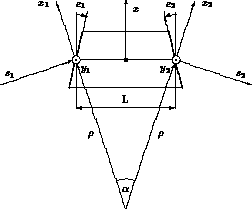
\includegraphics{figures/ref_rbend.png}
  \caption{Reference System for Rectangular Bends; The signs of the pole-face rotations are positive as shown.}
%\\\textbf{Figure 2:} Reference System for Rectangular Bends; The signs of the pole-face rotations are positive as shown. 
\end{figure}

%%\includegraphics{null}}
\begin{figure}[H]
  \centering
	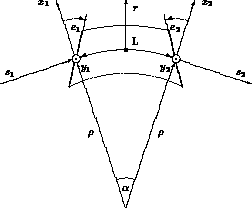
\includegraphics{figures/ref_sbend.png}
  \caption{Reference System for Sector Bends; The signs of the pole-face rotations are positive as shown. }
%\\\textbf{Figure 3:}  Reference System for Sector Bends; The signs of the pole-face rotations are positive as shown. 
\end{figure}


%\subsection{Elements which do not Change the Local Reference}
\subsection{Marker Elements}
\href{marker.html}{MARKER} elements do not  affect the reference orbit. 
They are ignored for geometry calculations.  

%\href{http://www.cern.ch/Hans.Grote/hansg_sign.html}{hansg}, January 24, 1997 
